\documentclass[a4paper]{article}
\usepackage[margin=0mm]{geometry}
\usepackage{tikz}
\pagestyle{empty}
\setlength{\parindent}{0pt}

% =====================================================
% SETTINGS
% =====================================================
\providecommand{\ExamTitle}{LINEAR ALGEBRA FINAL EXAM}
\providecommand{\NumQuestions}{100}          % Supported sizes: 10, 20, 30, 50, 100
\providecommand{\QuestionsPerColumn}{25}     % 25 gives: 20=1 col, 50=2 cols, 100=4 cols
\providecommand{\StudentDigits}{8}
\providecommand{\TestDigits}{4}

\providecommand{\IDBubbleR}{0.13}
\providecommand{\AnswerBubbleR}{0.145}
\providecommand{\ColumnW}{4.65}
\providecommand{\RowStep}{0.62}

\providecommand{\AnswerLeft}{1.25}
\providecommand{\AnswerRight}{19.75}
\providecommand{\AnswerTop}{20.65}
\providecommand{\AnswerBottom}{1.70}

% OpenCV ArUco DICT_4X4_50 markers with one black border bit.
% Corner IDs are assigned clockwise: 0=top-left, 1=top-right,
% 2=bottom-right, 3=bottom-left.
\def\ArucoSize{1.20}
\def\ArucoQuiet{0.15}

\newcommand{\DrawArucoCells}[3]{%
    \begin{scope}
        \pgfmathsetmacro{\cell}{\ArucoSize/6}
        \pgfmathsetmacro{\qxone}{#1-\ArucoQuiet}
        \pgfmathsetmacro{\qyone}{#2-\ArucoQuiet}
        \pgfmathsetmacro{\qxtwo}{#1+\ArucoSize+\ArucoQuiet}
        \pgfmathsetmacro{\qytwo}{#2+\ArucoSize+\ArucoQuiet}
        \fill[white] (\qxone,\qyone) rectangle (\qxtwo,\qytwo);
        \foreach \r/\c in {#3} {
            \pgfmathsetmacro{\xcell}{#1+\c*\cell}
            \pgfmathsetmacro{\ycell}{#2+\ArucoSize-(\r+1)*\cell}
            \fill[black] (\xcell,\ycell) rectangle ++(\cell,\cell);
        }
    \end{scope}
}

\newcommand{\DrawArucoIDZero}[2]{%
    \DrawArucoCells{#1}{#2}{%
        0/0,0/1,0/2,0/3,0/4,0/5,
        1/0,1/2,1/5,
        2/0,2/1,2/3,2/5,
        3/0,3/1,3/2,3/5,
        4/0,4/1,4/2,4/4,4/5,
        5/0,5/1,5/2,5/3,5/4,5/5%
    }%
}

\newcommand{\DrawArucoIDOne}[2]{%
    \DrawArucoCells{#1}{#2}{%
        0/0,0/1,0/2,0/3,0/4,0/5,
        1/0,1/1,1/2,1/3,1/4,1/5,
        2/0,2/5,
        3/0,3/2,3/3,3/5,
        4/0,4/2,4/4,4/5,
        5/0,5/1,5/2,5/3,5/4,5/5%
    }%
}

\newcommand{\DrawArucoIDTwo}[2]{%
    \DrawArucoCells{#1}{#2}{%
        0/0,0/1,0/2,0/3,0/4,0/5,
        1/0,1/1,1/2,1/5,
        2/0,2/1,2/2,2/5,
        3/0,3/1,3/2,3/4,3/5,
        4/0,4/3,4/5,
        5/0,5/1,5/2,5/3,5/4,5/5%
    }%
}

\newcommand{\DrawArucoIDThree}[2]{%
    \DrawArucoCells{#1}{#2}{%
        0/0,0/1,0/2,0/3,0/4,0/5,
        1/0,1/2,1/3,1/5,
        2/0,2/2,2/3,2/5,
        3/0,3/1,3/3,3/4,3/5,
        4/0,4/1,4/4,4/5,
        5/0,5/1,5/2,5/3,5/4,5/5%
    }%
}

\begin{document}

\noindent
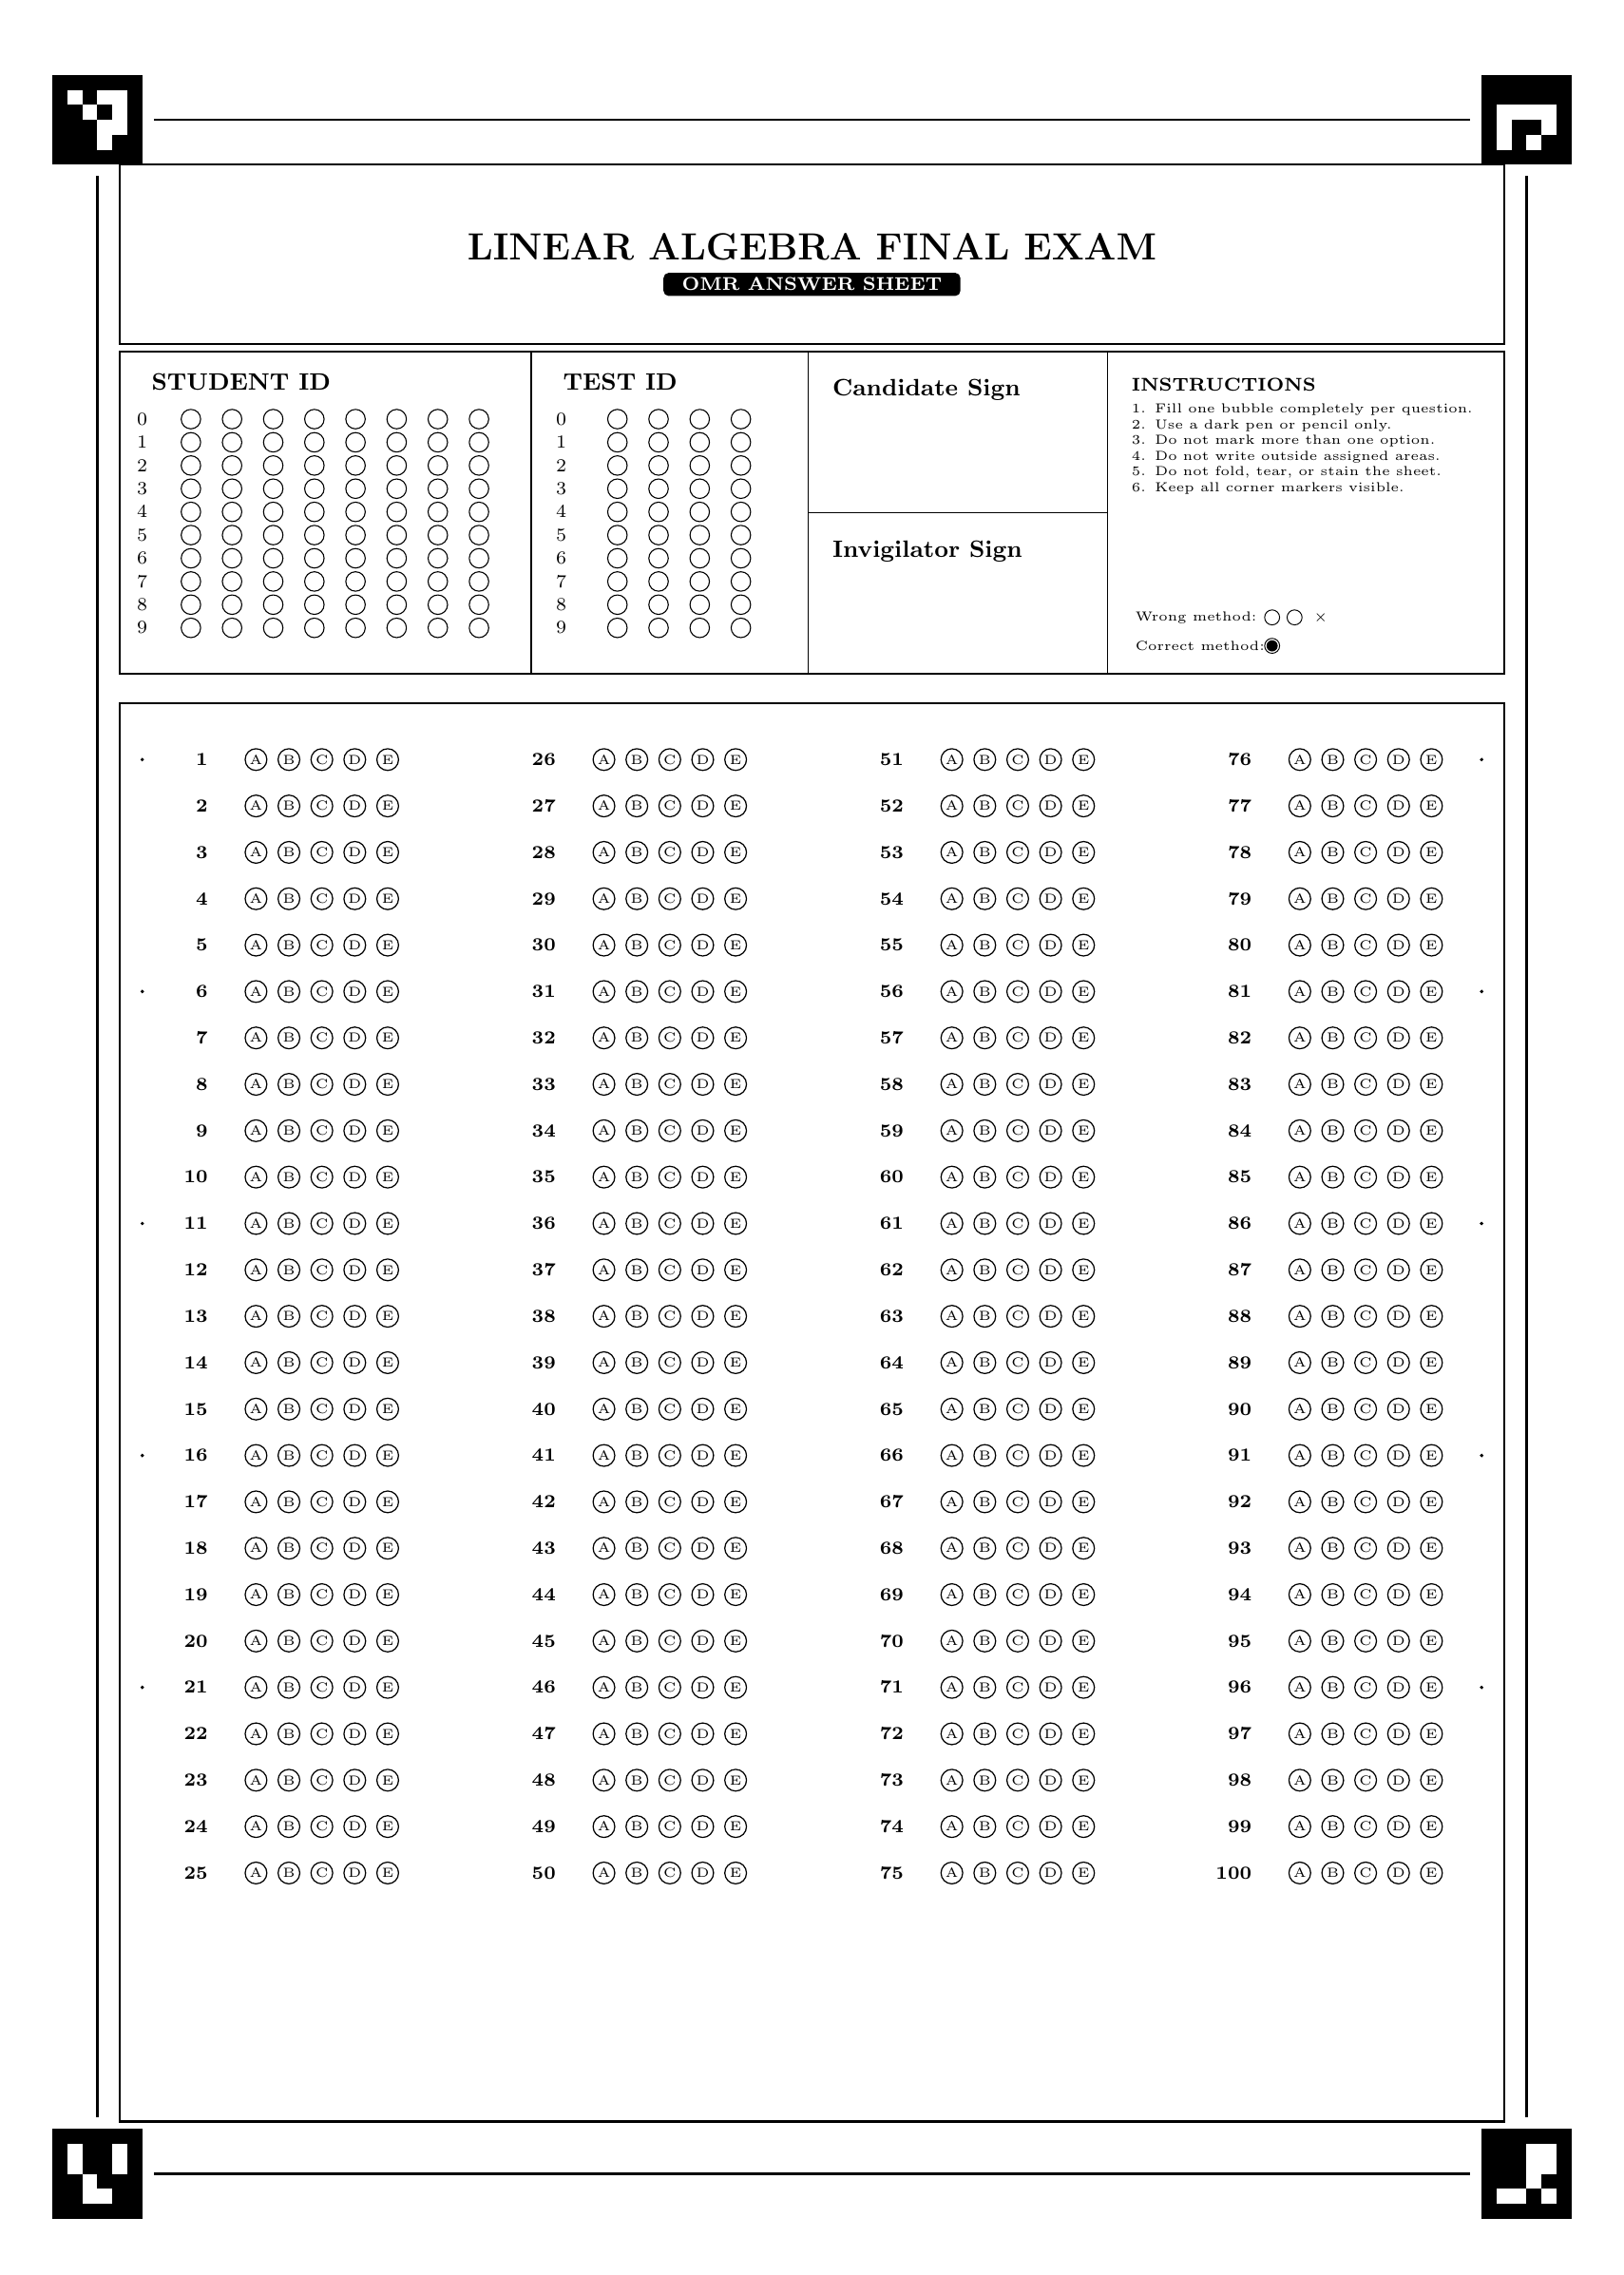
\begin{tikzpicture}[x=1cm,y=1cm]

% Page background
\fill[white] (0,0) rectangle (21,29.7);

% =====================================================
% OUTER FRAME
% =====================================================
\draw[line width=0.8pt] (0.95,1.0) rectangle (20.05,28.45);

% Four corner ArUco fiducials.
% The quiet white padding keeps the frame line from touching the marker.
\DrawArucoIDZero{0.35}{27.85}
\DrawArucoIDOne{19.45}{27.85}
\DrawArucoIDThree{0.35}{0.40}
\DrawArucoIDTwo{19.45}{0.40}

% =====================================================
% HEADER
% =====================================================
\draw[line width=0.7pt] (1.25,25.45) rectangle (19.75,27.85);

\node[font=\bfseries\Large] at (10.5,26.75) {\ExamTitle};

\node[
    fill=black,
    text=white,
    rounded corners=2pt,
    inner xsep=7pt,
    inner ysep=2pt,
    font=\bfseries\scriptsize
] at (10.5,26.25) {OMR ANSWER SHEET};

% =====================================================
% TOP INFORMATION AREA
% =====================================================
\draw[line width=0.7pt] (1.25,21.05) rectangle (19.75,25.35);
\draw[line width=0.7pt] (10.45,21.05) -- (10.45,25.35);

% =====================================================
% STUDENT ID AREA
% =====================================================
\draw[line width=0.6pt] (1.25,21.05) rectangle (6.75,25.35);
\node[anchor=west,font=\bfseries\small] at (1.55,24.95) {STUDENT ID};

\pgfmathtruncatemacro{\StudentDigitsMinusOne}{\StudentDigits - 1}

% Student ID bubbles: 0 to 9
\foreach \digit/\row in {0/0,1/1,2/2,3/3,4/4,5/5,6/6,7/7,8/8,9/9} {
    \pgfmathsetmacro{\y}{24.45 - \row*0.31}
    \node[font=\scriptsize] at (1.55,\y) {\digit};

    \foreach \i in {0,...,\StudentDigitsMinusOne} {
        \pgfmathsetmacro{\x}{2.20 + \i*0.55}
        \draw[line width=0.4pt] (\x,\y) circle (\IDBubbleR);
    }
}

% =====================================================
% TEST ID AREA
% =====================================================
\draw[line width=0.6pt] (6.75,21.05) rectangle (10.45,25.35);
\node[anchor=west,font=\bfseries\small] at (7.05,24.95) {TEST ID};

\pgfmathtruncatemacro{\TestDigitsMinusOne}{\TestDigits - 1}

% Test ID bubbles: 0 to 9
\foreach \digit/\row in {0/0,1/1,2/2,3/3,4/4,5/5,6/6,7/7,8/8,9/9} {
    \pgfmathsetmacro{\y}{24.45 - \row*0.31}
    \node[font=\scriptsize] at (7.15,\y) {\digit};

    \foreach \i in {0,...,\TestDigitsMinusOne} {
        \pgfmathsetmacro{\x}{7.90 + \i*0.55}
        \draw[line width=0.4pt] (\x,\y) circle (\IDBubbleR);
    }
}

% =====================================================
% SIGNATURE AND INSTRUCTIONS AREA
% =====================================================
\draw[line width=0.6pt] (10.45,21.05) rectangle (19.75,25.35);

% Signature boxes
\draw[line width=0.6pt] (10.45,23.2) rectangle (14.45,25.35);
\draw[line width=0.6pt] (10.45,21.05) rectangle (14.45,23.2);

\node[anchor=north west,font=\bfseries\small] at (10.65,25.1) {Candidate Sign};
\node[anchor=north west,font=\bfseries\small] at (10.65,22.95) {Invigilator Sign};

% Instructions box
\draw[line width=0.6pt] (14.45,21.05) rectangle (19.75,25.35);

\node[anchor=north west,font=\bfseries\scriptsize] at (14.65,25.12) {INSTRUCTIONS};

\node[
    anchor=north west,
    text width=4.85cm,
    align=left,
    font=\tiny
] at (14.65,24.78) {
1. Fill one bubble completely per question.\\
2. Use a dark pen or pencil only.\\
3. Do not mark more than one option.\\
4. Do not write outside assigned areas.\\
5. Do not fold, tear, or stain the sheet.\\
6. Keep all corner markers visible.
};

% Clean wrong/correct examples
\node[anchor=west,font=\tiny] at (14.70,21.80) {Wrong method:};
\draw[line width=0.35pt] (16.65,21.80) circle (0.10);
\draw[line width=0.35pt] (16.95,21.80) circle (0.10);
\node[font=\tiny] at (17.30,21.80) {$\times$};

\node[anchor=west,font=\tiny] at (14.70,21.42) {Correct method:};
\draw[line width=0.35pt] (16.65,21.42) circle (0.10);
\fill[black] (16.65,21.42) circle (0.075);

% =====================================================
% ANSWER AREA
% =====================================================
\draw[line width=0.8pt] (\AnswerLeft,\AnswerBottom) rectangle (\AnswerRight,\AnswerTop);

% Calculate number of columns
\pgfmathtruncatemacro{\Cols}{ceil(\NumQuestions / \QuestionsPerColumn)}
\pgfmathtruncatemacro{\ColsMinusOne}{\Cols - 1}

% Center the full group of columns safely inside the answer area.
\pgfmathsetmacro{\GroupW}{(\Cols - 1) * \ColumnW + 2.65}
\pgfmathsetmacro{\StartX}{(\AnswerLeft + \AnswerRight - \GroupW) / 2 + 0.35}

% Questions and bubbles
\foreach \q in {1,...,\NumQuestions} {

    \pgfmathtruncatemacro{\col}{floor((\q - 1) / \QuestionsPerColumn)}
    \pgfmathtruncatemacro{\row}{mod(\q - 1, \QuestionsPerColumn)}

    \pgfmathsetmacro{\x}{\StartX + \col*\ColumnW}
    \pgfmathsetmacro{\y}{19.90 - \row*\RowStep}

    % Question number, now safely inside the border
    \node[anchor=east,font=\bfseries\scriptsize] at (\x,\y) {\q};

    % Bubbles A B C D E
    \foreach \letter/\i in {A/0,B/1,C/2,D/3,E/4} {
        \pgfmathsetmacro{\bx}{\x + 0.52 + \i*0.44}

        \draw[line width=0.45pt] (\bx,\y) circle (\AnswerBubbleR);
        \node[font=\tiny] at (\bx,\y) {\letter};
    }
}

% =====================================================
% OPTIONAL CV-FRIENDLY REFERENCE DOTS
% Very small dots inside the answer region.
% Helpful for alignment, but not too intrusive.
% Comment this block if you want the sheet even cleaner.
% =====================================================
\foreach \r in {0,5,10,15,20} {
    \pgfmathsetmacro{\ty}{19.90 - \r*\RowStep}
    \fill[black] (1.55,\ty) circle (0.025);
    \fill[black] (19.45,\ty) circle (0.025);
}

\end{tikzpicture}

\end{document}
